\chapter{Definite Integrals with Substitutions}
\label{chap:1}
Focussing on the definite integral, $I =\int_{-\infty}^{+\infty}A\,\mathrm{d}x$. It brings up contradictory results as shown in proof.\ref{P1}
\begin{proof}[Proof 1]\label{P1}
	If $$A > 0, \implies I = \int_{-\infty}^{+\infty}A\,\mathrm{d}x \to \infty$$
	but if we break up the integral as in,
	$$I = \int_{-\infty}^{+\infty}A\,\mathrm{d}x = \int_{-\infty}^{-1}A\,\mathrm{d}x + \int_{-1}^{+1}A\,\mathrm{d}x + \int_{+1}^{+\infty}A\,\mathrm{d}x$$
	$$\implies I = 2A + \int_{-\infty}^{-1}A\,\mathrm{d}x + \int_{+1}^{+\infty}A\,\mathrm{d}x$$
	Substituting $$x = \frac{1}{y}\, \implies \mathrm{d}x = -\frac{1}{y^2} \mathrm{d}y$$
	We get;
	$$I = 2A +A\int_{-1}^{0} \frac{1}{y^2}\,\mathrm{d}y +A\int_{0}^{1} \frac{1}{y^2}\,\mathrm{d}y = 2A + A\int_{-1}^{1}\frac{1}{y^2}\,\mathrm{d}y$$
	$$\implies I = 2A + A(\frac{1}{y}\bigg\rvert_{1}^{-1}) = 0 $$
\end{proof}
The problem seems to be with the integral $I' = \int_{-1}^{+1}\frac{1}{y^2}\,\mathrm{d}y$. But, if we break it up into two integrals as shown in proof.\ref{P2}, Then the entire integral diverges as expected.
\begin{proof}[Proof 2]\label{P2}
	$$I' = \int_{-1}^{+1}\frac{1}{y^2}\,\mathrm{d}y$$
	\begin{align*}
		& = \int_{-1}^{0^-}\frac{1}{y^2}\,\mathrm{d}y + \int_{0^+}^{+1}\frac{1}{y^2}\,\mathrm{d}y \\
		& = -\bigg(\, \frac{1}{y}\bigg\rvert_{-1}^{0^-} + \frac{1}{y}\bigg\rvert_{0^+}^{+1}\,\bigg)\\
		& \to +\infty &&
	\end{align*}
\end{proof}
It is also to be noted that the divergence of the integral $I'$ is expected because as can be seen from proof.\ref{P1}, $I = 2A + I'$ and $I \to \infty$, hence it has to logically follow that $I' \to \infty$. But, it is noteworthy looking at the graph of fig.\ref{F1a} which shows the increase in the integral area $I'$ around the point $x=0$.
\begin{figure}[h]
	\centering
	\begin{subfigure}[t]{0.49\textwidth}
		\centering
		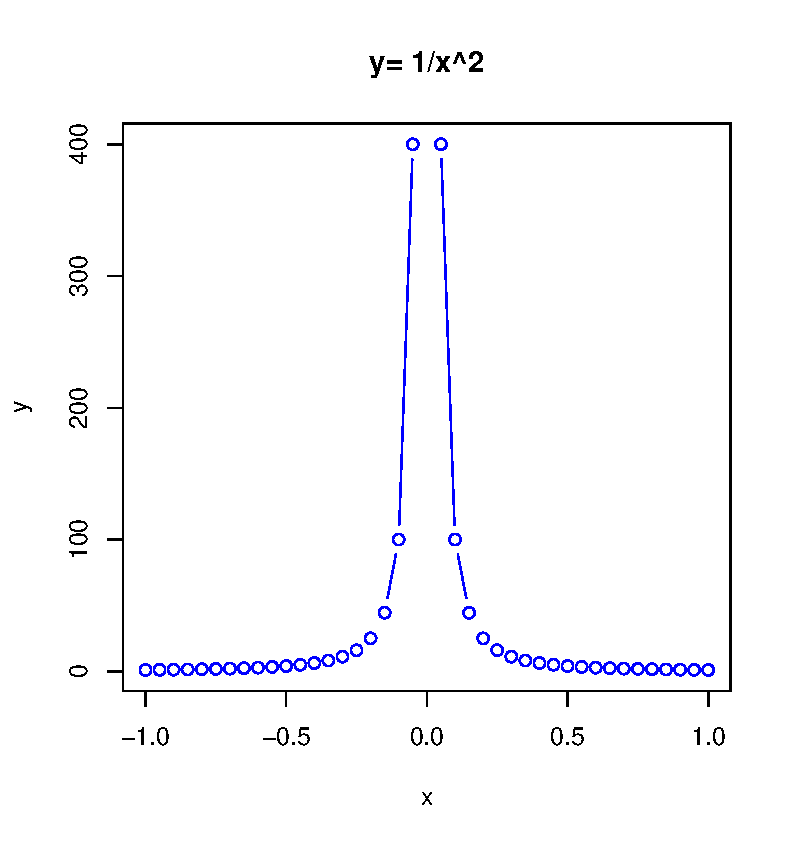
\includegraphics[width=\linewidth]{Plot1a.pdf}
		\phantomsubcaption
		\label{F1a}
	\end{subfigure}
	\hfill
	\begin{subfigure}[t]{0.49\textwidth}
		\centering
		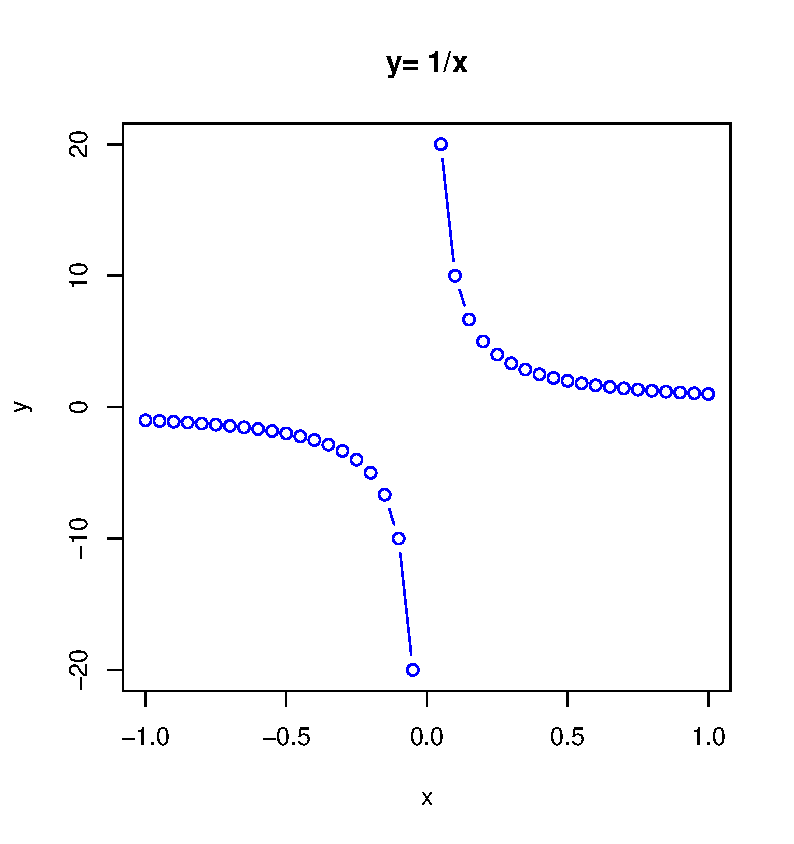
\includegraphics[width=\linewidth]{Plot1b.pdf}
		\phantomsubcaption
		\label{F1b}
	\end{subfigure}
	\caption{(a)Plot of $y=1/x^2$ generated using R. (b)Plot of $y = 1/x$ generated using R.}\label{F1}
\end{figure}
It is noteworthy to see that since $\lim_{x \to 0^-}1/x^2 = \lim_{x \to 0^+}1/x^2$, hence there is no discontinuity at the point $x = 0$, but it is important to note that the antiderivative $1/x$ is discontinuous at $x=0$ as seen in fig.\ref{F1b}, and also the function $1/x^2$ is not differentiable at the point $x=0$ since the derivative of $1/x^2$ is $-2/x^3$ and the derivative is not continuous at $x=0$, that is, the $\lim_{x \to 0^-} 2/x^3 \neq \lim_{x \to 0^+}2/x^3$.\\

To answer the question as to why the discontinuity of the antiderivate matters for an integral taken over the interval containing the point in question, we need to look closely at the \textit{fundamental theorum of calculus} talked about in \autoref{chap:2}.